\input{configuration}

\title{Lecture 33 --- Trusted Computing}

\author{Jeff Zarnett \\ \small \texttt{jzarnett@uwaterloo.ca}}
\institute{Department of Electrical and Computer Engineering \\
  University of Waterloo}
\date{\today}


\begin{document}

\begin{frame}
  \titlepage
\end{frame}


\begin{frame}
\frametitle{Trusted Computing}

\begin{center}
	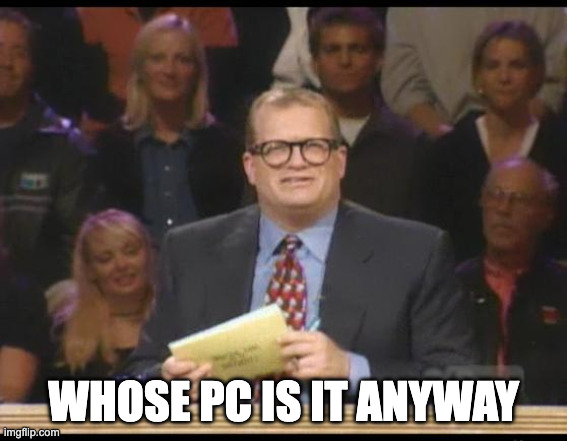
\includegraphics[width=0.4\textwidth]{images/whosepc.jpg}
\end{center}

Previously: online multiplayer games use kernel-level anti-cheat mechanisms.

\end{frame}


\begin{frame}
\frametitle{Trusted Computing}

\begin{center}
	
\includegraphics[width=0.4\textwidth]{images/deeper.jpg}
\end{center}

In 2025, for example, Activision/Blizzard announced that they would require TPM 2.0 and Secure Boot to play Call of Duty.

These two are hardware-based functionality that are ostensibly about security.

\end{frame}

\begin{frame}
\frametitle{The History Lesson}


The focus on hardware-level protection of what is allowed to run on the computer started around the year 2000. 

That year: the publication of the version 1.0 specification of Trusted Computing. 

It is \textit{not at all} a coincidence that this conversation started at a time where the hot topic amongst the megacorporations was ``stopping music piracy''.

\end{frame}


\begin{frame}
\frametitle{The History Lesson}

\begin{center}
	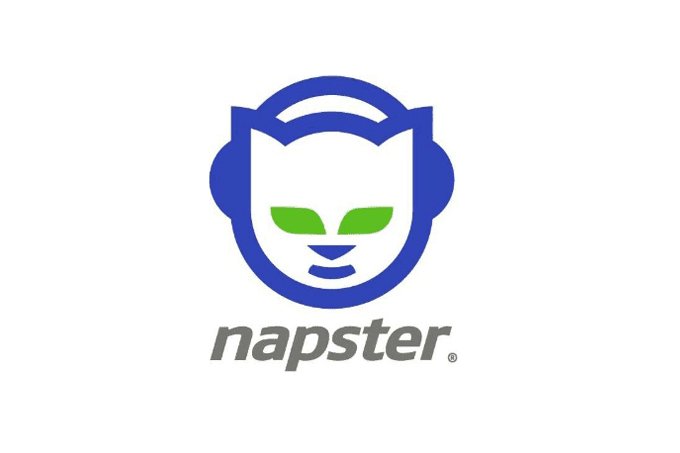
\includegraphics[width=0.7\textwidth]{images/napster.png}
\end{center}

In June of 1999, the application Napster launched: Peer-to-Peer music sharing.

\end{frame}


\begin{frame}
\frametitle{DRM}

The big players looked to stop this through \alert{Digital Rights Management (DRM)}.

DRM: The ability to stop you from doing things they do not want you to do with the media that you purchased. 

It is really \textit{digital restrictions management}.

\end{frame}


\begin{frame}
\frametitle{DRM}

These restrictions only work if the software understands what you are and are not allowed to do, and enforces those constraints. 

\begin{center}
	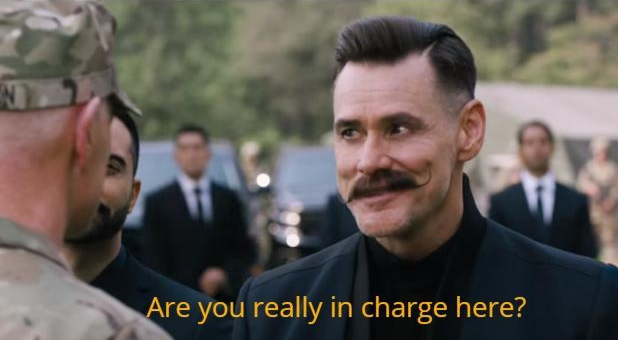
\includegraphics[width=0.5\textwidth]{images/incharge.jpg}
\end{center}

You can very likely think of some workarounds for these restrictions immediately, if you control the computer and its software.

\end{frame}


\begin{frame}
\frametitle{Legal Disclaimer}

Circumvention of DRM restrictions is a legal minefield! 

There exist valid reasons and circumstances where it is your legal right to do so, and other circumstances where the same actions are a violation of copyright law. 

Consult a lawyer to learn the specifics. 
\begin{center}
	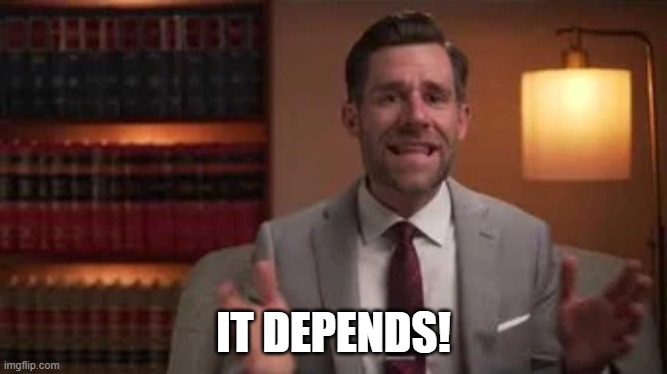
\includegraphics[width=0.5\textwidth]{images/legaleagle.jpg}
\end{center}

\end{frame}


\begin{frame}
\frametitle{DRM Circumvention}

\begin{center}
	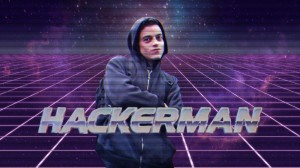
\includegraphics[width=0.4\textwidth]{images/hackerman.jpg}
\end{center}

Edit the binary to change the if-else condition?

Find the encryption key in process memory?

Redirect network call?

Load your own kernel module?

\end{frame}




\begin{frame}
\frametitle{Arms Race}

 The key factor in all of the examples given above? 
 
 The person who purchased and administers the computer has a lot of ability to modify application software and even the OS.

They're not trivial, but once is enough.

\end{frame}



\begin{frame}
\frametitle{Arms Race}

The prevention of circumvention of DRM has to move down, into hardware.

That's the only way to break that condition where the administrator of the computer has enough control to bypass restrictions.


\end{frame}


\begin{frame}
\frametitle{TC Quote}

\begin{quote}
TC provides a computing platform on which you can't tamper with the application software, and where these applications can communicate securely with their authors and with each other. The original motivation was digital rights management (DRM): Disney will be able to sell you DVDs that will decrypt and run on a TC platform, but which you won't be able to copy. The music industry will be able to sell you music downloads that you won't be able to swap. They will be able to sell you CDs that you'll only be able to play three times, or only on your birthday.
\end{quote}
\hfill -- Ross Anderson

\end{frame}


\begin{frame}
\frametitle{And Then, It Got Worse}

The current state of DRM is that it allows the corporation to alter the deal at any time. 

In 2026, for example, Sony deleted movies (including T2!) that customers paid for.

\begin{center}
	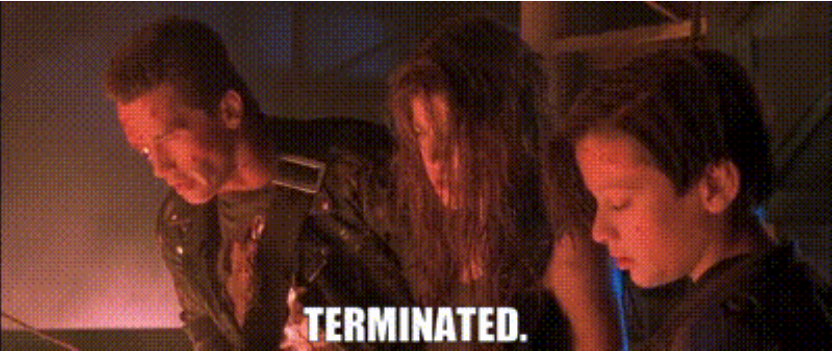
\includegraphics[width=0.5\textwidth]{images/isitdead.png}
\end{center}

Yes, yes, licensing vs ownership. But they \textit{can} do this.

\end{frame}


\begin{frame}
\frametitle{Hardware Solution}

If I control the kernel -- including live-patching it -- I can bypass restrictions. 

What if the computer refuses to boot a kernel that is not ``approved''?\\
\quad... And such an approved kernel would forbid any live-patching!

(People will find a way.)

\end{frame}


\begin{frame}
\frametitle{Not Just Anti-Piracy}

This can go beyond preventing people from watching media or copying software.

It can be used to delete content that the government, or other powerful actors, don't want you to have. 

The standard dystopian example of this: imagine a journalist has published an expos\'e on the corruption and criminality of the dictator of a country.

What if the dictator simply has the ability to order that all copies of that document are deleted from everyone's computer?

\end{frame}


\begin{frame}
\frametitle{Not Useless}

At least at present, if verification fails, the computer is not useless...

It's just in an \alert{untrusted} state.

You can do a lot... but not play the desired game or consume restricted media.

\end{frame}


\begin{frame}
\frametitle{More Useless}

It is, however, not unthinkable that the future state is that it will be difficult to run the computer in an untrusted state at all.

As life becomes increasingly conducted online, it gets harder over time to use a ``free'' computer if you cannot use it to do the things needed in everyday life.

Examples: online banking, pay tax, order online, edit documents...

\end{frame}


\begin{frame}
\frametitle{Quixotic Quest}

It is also important to note that perfection on digital restrictions like this is impossible for multiple reasons.

One of them is referred to as ``the analog hole''.

\begin{center}
	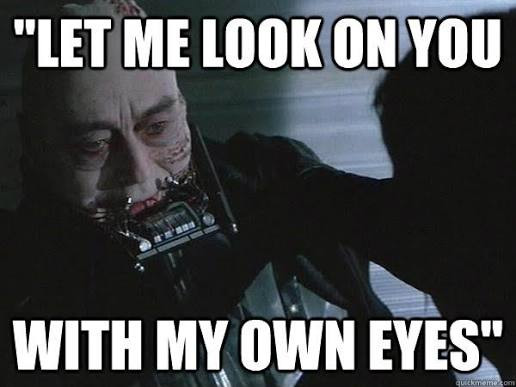
\includegraphics[width=0.4\textwidth]{images/owneyes.jpg}
\end{center}

People will find a way; it's just a question of how hard it is. 

\end{frame}


\begin{frame}
\frametitle{Say No to Brain Implants, Kids}

Under no circumstances should you let anybody put a chip in your brain to ``permit'' you to watch restricted content.

\begin{center}
	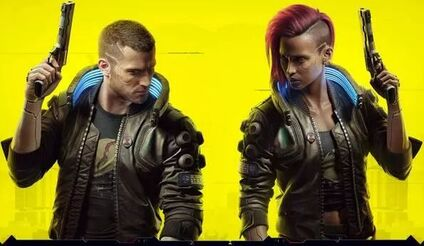
\includegraphics[width=0.4\textwidth]{images/v-cyberpunk.jpg}
\end{center}

The future where media companies are inside your brain is corporate serfdom, not Cyberpunk 2077.

\end{frame}


\begin{frame}
\frametitle{Alternative Uses}

Gaming provides a legitimate example. 

The kernel-level anti-cheat module can be backstopped by the trusted computing platform.

\end{frame}



\begin{frame}
\frametitle{War Thunder}

There are also scenarios where locking down documents may serve reasonable government or military purposes.

\begin{center}
	
\includegraphics[width=0.4\textwidth]{images/warthunder.jpeg}
\end{center}

\end{frame}


\begin{frame}
\frametitle{Kernel Compromise}

If malware is installed in the system firmware or boot loader, the malware can survive if the OS is reinstalled.

The OS cannot find it, because the OS is running itself on a compromised foundation. 

\begin{center}
	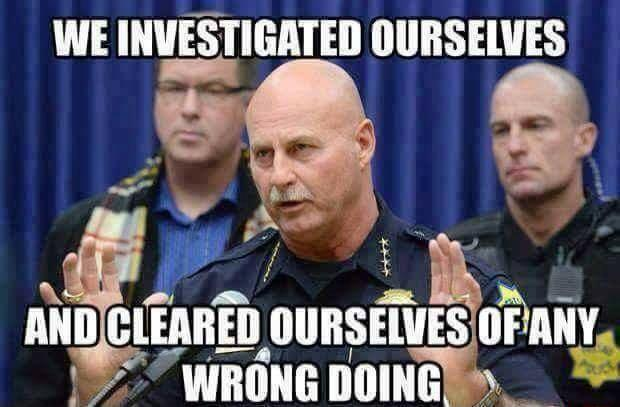
\includegraphics[width=0.4\textwidth]{images/wrongdoing.jpeg}
\end{center}

This is a \alert{bootkit}.

\end{frame}


\begin{frame}
\frametitle{Secure Boot}

The supposed solution to that is called \alert{Secure Boot}.

It is a security feature in the UEFI standard to verify these low-level foundational components to be sure they are valid.


Verify first, and then transfer control.

\end{frame}

\begin{frame}
\frametitle{Nothing's Perfect}

There are numerous examples of bypassing secure boot.\\
\quad Example: BlackLotus from 2022. 

This malware uses a known vulnerability to bypass secure boot, and exactly like the driver revocation problem we discussed.

\end{frame}


\begin{frame}
\frametitle{Access Denied}

Alongside the idea of secure boot is \alert{measured boot}. 

Instead of just allow or deny kind of semantics, measured boot hashes and records the state of the things that ran, whether that's been altered or not.

Change detection!

\end{frame}


\begin{frame}
\frametitle{Measured Boot}

Arch Linux: these measured boot values can also be used as a gating function for whether access is permitted. 

We need some hardware support: the \alert{Trusted Platform Module (TPM)}


The TPM permits management of encryption keys.

\end{frame}


\begin{frame}
\frametitle{TPM Example: Encrypt Drive}

Suppose the boot drive of the system is encrypted. 

The encryption key will be sealed by the hardware TPM.

The module will release the encryption key only if the assessment of the boot state is acceptable.

But it also needs to handle change!

\end{frame}


\begin{frame}
\frametitle{Attestation}

We've discussed two ways in which the state of the system can be assessed.

Do those checks produce reliable results?

\begin{center}
	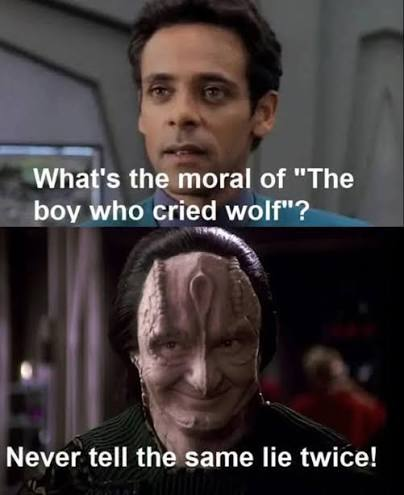
\includegraphics[width=0.4\textwidth]{images/garak.jpg}
\end{center}

\end{frame}


\begin{frame}
\frametitle{Attestation}

The solution is called \alert{attestation}: verifying, externally, the claims.

Attestation has a few steps:

\begin{enumerate}
	\item Measurement: collect evidence.
	\item Request verification from remote system.
	\item Challenger/appraiser sends random one-time code.
	\item Combine this code with measurement.
	\item Use TPM to sign using TPM signing key.
	\item Send to challenger and verify.
	\item If signature, one-time code, and measurement are valid: pass.
\end{enumerate}


\end{frame}


\begin{frame}
\frametitle{Attestation}

For the game, inspect the state of the system.\\
\quad Pass means you can launch the game.

Probably there are periodic re-checks? Kick if failed?

\end{frame}


\begin{frame}
\frametitle{Attestation}

Get around the problem of self-report; external validation.

The validator is not under the control of the bad actors.

We should view the threat model from the view of the game server.

\end{frame}


\begin{frame}
\frametitle{Attestation}

The one-time code prevents replaying an old response.

The cryptographic signing is hard to forge because only the machine's TPM has the (unique) signing key.

Validating the signing key is farther down the cryptography and security track than we consider to be in-scope for this course.

\end{frame}


\begin{frame}
\frametitle{Attestation}

We forgot to talk about one thing, though: how can we be sure that the measurement is valid? 

Remember that verification happens at each stage, before we go on to the next. 

If we start from a secure place, like the UEFI, it will accurately record the boot loader's measurement. 

If the kernel is compromised, that compromise has already been recorded before it gets a chance to run. 

And the record cannot be rewritten by a malicious kernel.

\end{frame}


\begin{frame}
\frametitle{Rewrite the Record?}

That just moves the problem one step along: why can the kernel not rewrite the record? 

The TPM does not offer that functionality!\\
\quad Read, Reset, Extend.


\end{frame}


\begin{frame}
\frametitle{Chain of Trust}

All of this might make you feel a certain level of concern as to what exactly is going on in the devices that you allegedly own.

There are so many points at which a bad actor could compromise the security.

\end{frame}


\begin{frame}
\frametitle{Chain of Trust}

Part of the argument for open-source software is that you can, at least in principle, audit the code in it.

Closed source can be audited too, with more difficulty.

But it is a huge undertaking!


\end{frame}


\begin{frame}
\frametitle{Cloud Computing}

The problem is worse in the world of cloud computing.

\begin{center}
	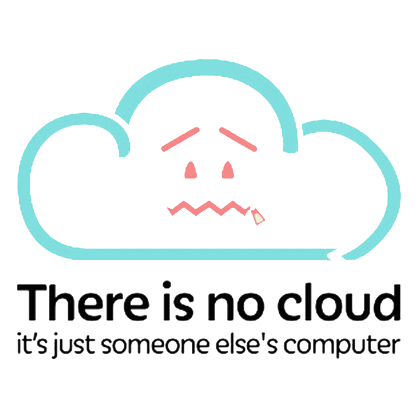
\includegraphics[width=0.25\textwidth]{images/cloud.png}
\end{center}

 Cloud computing is rather diametrically opposed to that view: you own nothing, but instead rent some resources from the cloud provider. 
 
 So you need to trust the cloud provider, its hardware, its hypervisor, or the people who run the cloud computing platform in general. 

\end{frame}


\begin{frame}
\frametitle{Near-Miss}

 Early in 2024, a compromise was discovered in the \texttt{xz} library.
 
 The library is used for data compression; some versions of \texttt{openssh} rely on it. 
 
 This is a strong example of what's termed a ``supply chain attack''. 


\end{frame}

\begin{frame}
\frametitle{Near-Miss}

Almost any modern piece of software that isn't a toy or academic assignment is built in a compositional way. 

$A$ uses libraries $B, C, D$ each of which has dependencies $E, F, G, H...$

Compromising any one of the dependencies $F$ could result in a vulnerability in $A$. 

But if $A$ is \texttt{openssh}, you know, the \textit{secure} shell daemon...
\end{frame}



\begin{frame}
\frametitle{Near-Miss}


And yet, it's worse than that. 

The compromise of the library was in the build system for \texttt{xz}, not the code itself. 

Merely examining the source of the library wouldn't have found the problem.

\end{frame}


\begin{frame}
\frametitle{Bad Things or Bad Actors}

Ken Thompson told us in a 1984 lecture that you cannot trust code that you did not write yourself or that's built using a toolchain that you did not write.

We have to put some trust in \textit{some people}, otherwise we will never be able to accomplish anything. 

\end{frame}


\begin{frame}
\frametitle{Bad Things or Bad Actors}

It feels bad, in a way, to say that we have to just trust other people.\\
\quad After all: \textit{we live in a society.}

Obviously, a battery-powered drill won't leak your health records to hackers...

You're still counting on it to not explode in your hands or burn your home down.

Trust is fundamental to society. Look skeptically at software you did not write.\\
\quad Do so proportionally with the magnitude of risks.

\end{frame}




\end{document}
